% Komplexní sdružení
% P. Kulhánek, ‘O vztahu matematiky a fyziky,’ 2018. WWW: 
% https://1drv.ms/b/s!Ajq2sO-eH2xUhpIEk1mJBg4c0TrlF

% https://tex.stackexchange.com/questions/247541/

\documentclass[11pt, border=2pt]{standalone}
  \usepackage{pgf,tikz,pgfplots}
    \pgfplotsset{compat=1.15}
    \usetikzlibrary{arrows}
    \usetikzlibrary{calc}
  \usepackage{amsmath}

    \begin{document}
        \definecolor{blue}{rgb}{0,0,1}
        \definecolor{red}{rgb}{0.8,0,0}
        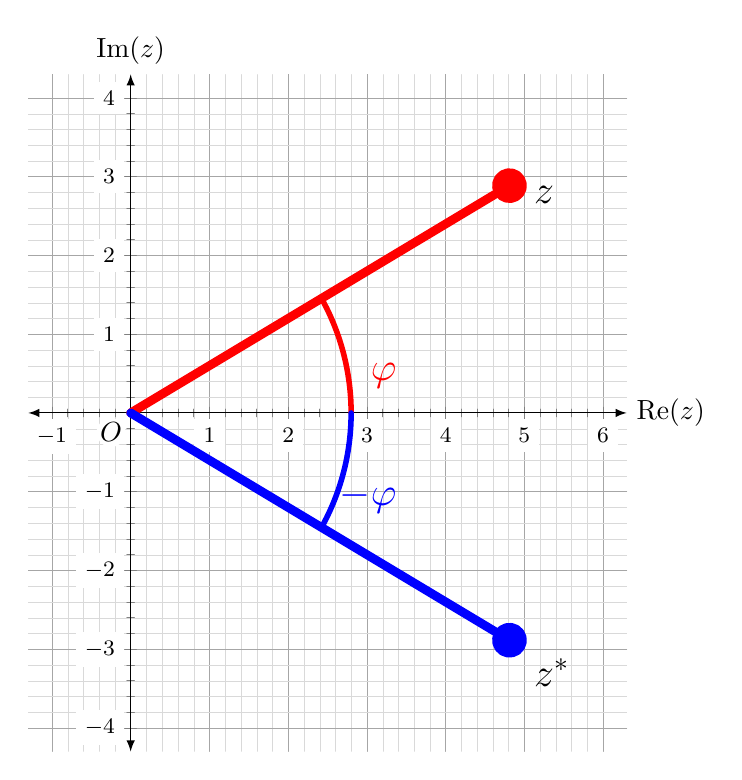
\begin{tikzpicture}[line cap=round,line join=round,>=triangle 45,x=1cm,y=1cm]
            \begin{axis}[
                x=1cm, 
                y=1cm,
                axis lines=middle,
                ymajorgrids=true,
                xmajorgrids=true,
                xmin=-1.1,
                xmax=6.1,
                ymin=-4.1,
                ymax=4.1,
                xtick={-1,0,1,...,6},
                ytick={-4,-3,...,4},
                grid=both,
                grid style={line width=.1pt, draw=gray!30},
                major grid style={line width=.2pt,draw=gray!70},
                minor tick num=4,
                xlabel style={at={(ticklabel* cs:1)},anchor=west},
                ylabel style={at={(ticklabel* cs:1)},anchor=south},
                ticklabel style={font=\footnotesize,fill=white},
                axis line style={latex-latex},
                xlabel={$\operatorname{Re}(z)$},
                ylabel={$\operatorname{Im}(z)$},
                enlargelimits={abs=0.2}
            ]
            \coordinate (O) at (0,0);
            \node[fill=white,circle,inner sep=0pt] (O-label) at ($(O)+(-135:10pt)$) {$O$};
            
            \draw [-*, line cap=round, line width=3.2pt,color=red]  (0,0) -- (5,3);
            \draw [-*, line cap=round, line width=3.2pt,color=blue] (0,0) -- (5,-3);
            \draw [shift={(-1.3,-4.1)},line width=2pt,color=red]  
                plot[domain=0:0.5,variable=\t]({1*3*cos(\t r)+0*3*sin(\t r)},{0*3*cos(\t r)+1*3*sin(\t r)});
            \draw [shift={(-1.3,-4.1)},line width=2pt,color=blue]  
                plot[domain=-0.5:0,variable=\t]({1*3*cos(\t r)+0*3*sin(\t r)},{0*3*cos(\t r)+1*3*sin(\t r)});
            \draw (5,+3) node[anchor=north west] {\Large$z$};
            \draw (5,-3) node[anchor=north west] {\Large$z^*$};
            \draw (3.5,+0.75) node[anchor=north east, color=red] {\Large$\varphi$};
            \draw (3.5,-0.75) node[anchor=north east, color=blue] {\Large$-\varphi$};
            % \draw [line width=3.2pt,color=red] (2,0) arc (0:45:1);
            % \draw [line width=3.2pt,color=blue] (2,0) arc (0:-45:1);
            \end{axis}
        \end{tikzpicture}
    \end{document}